\section{Dichotomie}
\begin{enumerate}[(a)]
  \item \q{Ecrire une fonction récursive }\il{dicho(f, a, b, eps)}\q{ qui
          calcule par dichotomie la racine de $f$ entre $a < b$ sachant que $f$
          est continue et $f(a)\times f(b) < 0$ à une erreur eps près.}

        Avant tout j'importe \il{numpy} et \il{pylab} :
        \codeFromFile{section-02/qa-1.py}
        Puis je code la fonction demandée :
        \codeFromFile{section-02/qa-2.py}
  \item \q{Par exemple, trouver les trois racines de $P(x) = x^3 -3x - 1$ à }
        \il{eps}
        \q{ = $10^{-5}$ près.}

        \begin{dinglist}{111}
          \item
          D'abord je trace la fonction à étudier :
          \codeFromFile{section-02/qb-2.py}
          \begin{center}
            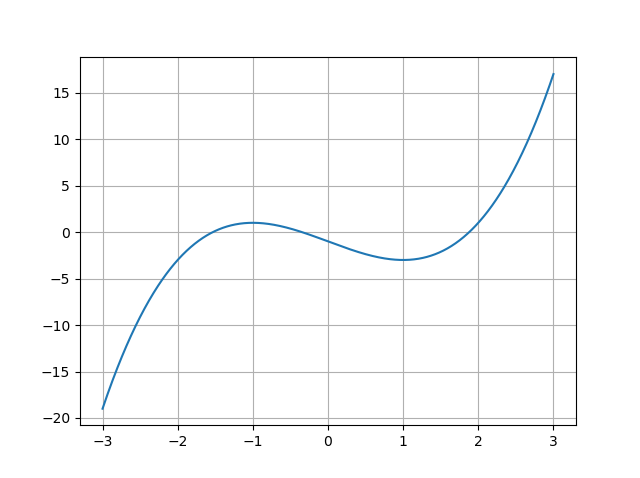
\includegraphics[scale=0.5]{section-02/qb-3.png}
          \end{center}

          \item
          Je note grossièrement les 3 intervalles contenant les racines, et la
          précision de recherche :
          \codeFromFile{section-02/qb-4.py}

          \item
          Je calcule les racines à $10^{-5}$ près :
          \codeFromFile{section-02/qb-5.py}
          Je trouve :
          \[
            \left\{
            \begin{array}{rcl}
              \alpha & = & \il{-1.5320816040039062}  \\
              \beta  & = & \il{-0.34729766845703125} \\
              \gamma & = & \il{1.8793869018554688}   \\
            \end{array}
            \right.
          \]
        \end{dinglist}


  \item \q{On reprend l'exemple du DS 3 :}
        \[
          R =
          \left(
          \begin{array}{ccc}
              0 & 0 & 1 \\
              1 & 0 & 3 \\
              0 & 1 & 0 \\
            \end{array}
          \right)
        \]
        \q{Définir les matrice $R$ et $D$ diagonales telles que  $R$ semblable à
          $D$ ainsi que la matrice de passage $P$. Calculer par la
          diagonalisation $M^{10}$ et vérifier que l'erreur sur
          les coefficients est en pourcentage des plus grands coefficients de
          l'ordre de $eps$.}\\
        \q{Vérifier que l'erreur pour $M^n$ est de l'ordre de $\frac{n}{10}eps$
          pour $n\in \{20; 50; 100; 1000\}$}

        \begin{dinglist}{111}
          \item
          J'ai :

          \[
            \begin{array}{ccc}

              R =
              \left(
              \begin{array}{ccc}
                  0 & 0 & 1 \\
                  1 & 0 & 3 \\
                  0 & 1 & 0 \\
                \end{array}
              \right)

               &

              D =
              \left(
              \begin{array}{ccc}
                  \alpha & 0     & 0      \\
                  0      & \beta & 0      \\
                  0      & 0     & \gamma \\
                \end{array}
              \right)

               &

              P =
              \left(
              \begin{array}{ccc}
                  1        & 1       & 1        \\
                  \alpha^2 & \beta^2 & \gamma^2 \\
                  \alpha   & \beta   & \gamma   \\
                \end{array}
              \right)
            \end{array}
          \]
          De plus, $M = PDP^{-1} \Rightarrow M^n=PD^nP^{-1}$ avec $M=R$ à
          $10^{-5}$ près.

          \item
          Je définit la fonction \il{getRPowN} qui calcule $M^n=PD^nP^{-1}$ :
          \codeFromFile{section-02/qc-1.py}

          \newpage


          \item
          De même, je définit la fonction \il{puiss} qui calcule $R^n$ :
          \codeFromFile{section-02/qc-2.py}

          \item
          Je définit la fonction qui calcule l'erreur en pourcentage :
          \codeFromFile{section-02/qc-3.py}

          \item
          Je calcule l'erreur pour \il{n = 10} et trouve \il{1.62 \%},
          ce qui correspond à ce qu'il fallait trouver.


          \item
          Je recommence, mais $n$ fois, avec $n\in\{20, 50, 100, 1000\}$, et je
          trace les résultats :
          \codeFromFile{section-02/qc-4.py}

          \il{TraceError([20, 50, 100, 1000])} donne une droite de pente $\frac{eps}{10}$ :

          \begin{center}
            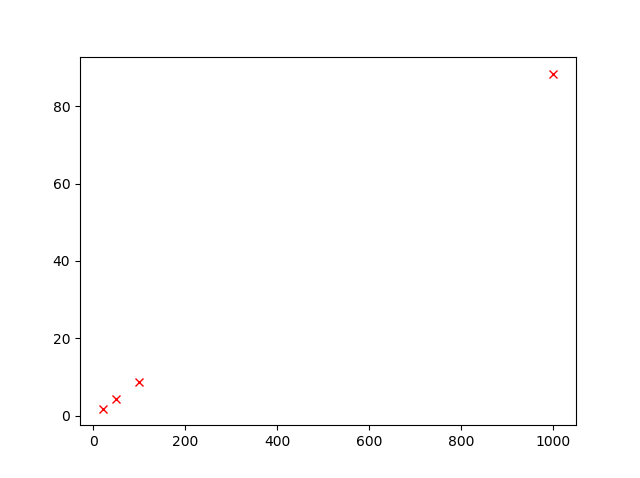
\includegraphics[scale=0.5]{section-02/qc-6.png}
          \end{center}

        \end{dinglist}
\end{enumerate}
